\documentclass{standalone}
\usepackage{tikz}
\usetikzlibrary{patterns, positioning}

\begin{document}
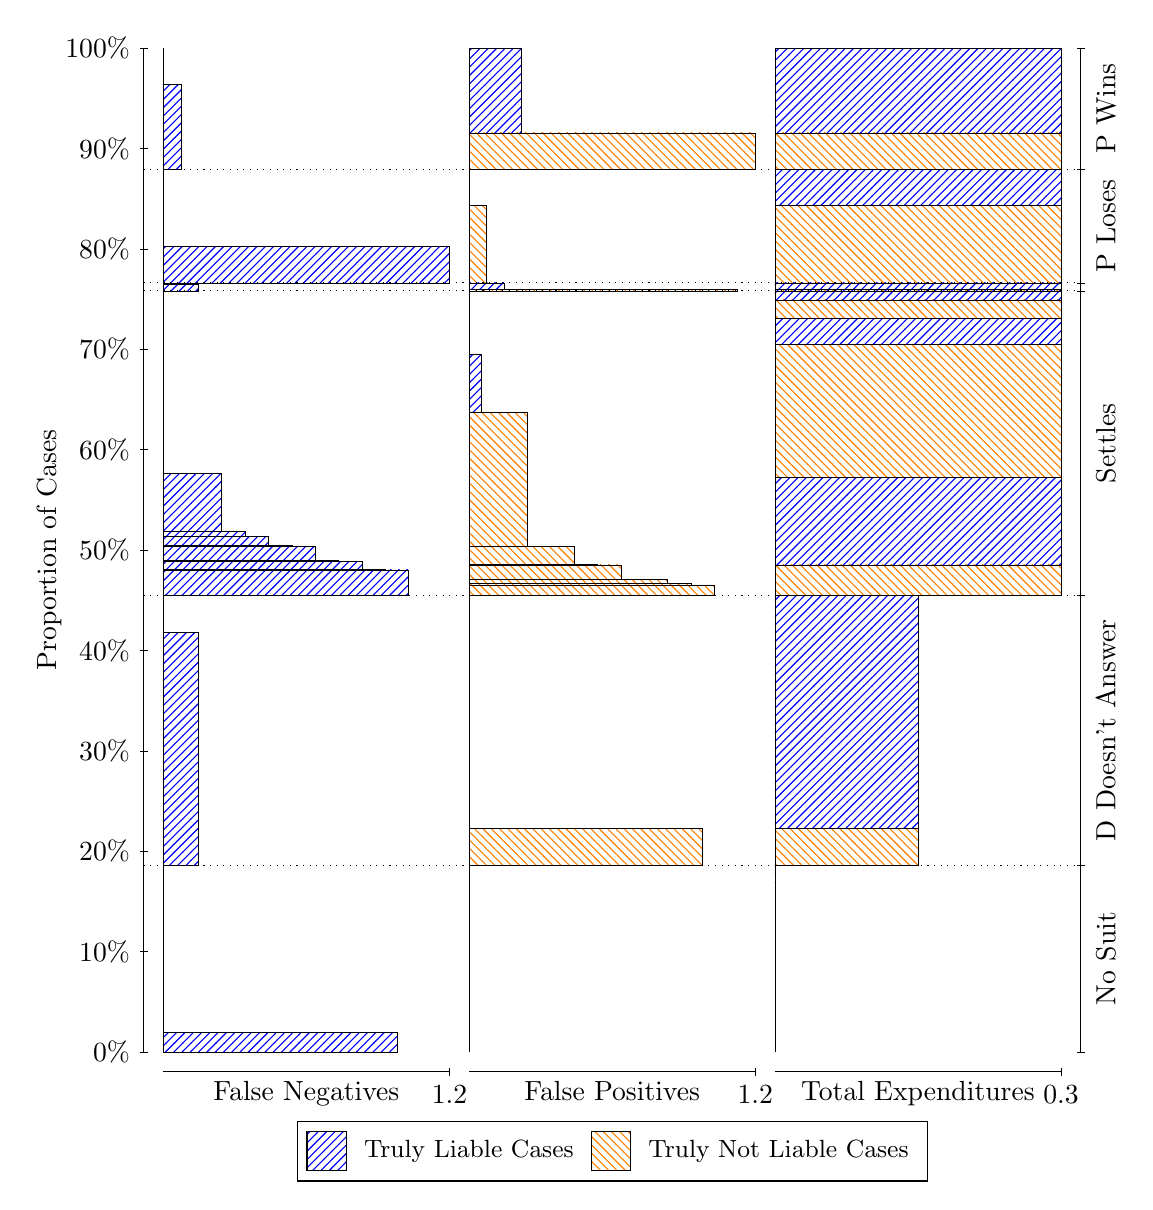
\begin{tikzpicture}
\draw[black, very thin] (1.5,1.75) -- (1.5,14.5);
\node[rotate=90, anchor=center] at (0.3, 8.125) {Proportion of Cases};
\draw[black, very thin] (1.45,1.75) -- (1.55,1.75);
\node[anchor=east] at (1.45, 1.75) {0\%};
\draw[black, very thin] (1.45,3.025) -- (1.55,3.025);
\node[anchor=east] at (1.45, 3.025) {10\%};
\draw[black, very thin] (1.45,4.3) -- (1.55,4.3);
\node[anchor=east] at (1.45, 4.3) {20\%};
\draw[black, very thin] (1.45,5.575) -- (1.55,5.575);
\node[anchor=east] at (1.45, 5.575) {30\%};
\draw[black, very thin] (1.45,6.85) -- (1.55,6.85);
\node[anchor=east] at (1.45, 6.85) {40\%};
\draw[black, very thin] (1.45,8.125) -- (1.55,8.125);
\node[anchor=east] at (1.45, 8.125) {50\%};
\draw[black, very thin] (1.45,9.4) -- (1.55,9.4);
\node[anchor=east] at (1.45, 9.4) {60\%};
\draw[black, very thin] (1.45,10.675) -- (1.55,10.675);
\node[anchor=east] at (1.45, 10.675) {70\%};
\draw[black, very thin] (1.45,11.95) -- (1.55,11.95);
\node[anchor=east] at (1.45, 11.95) {80\%};
\draw[black, very thin] (1.45,13.225) -- (1.55,13.225);
\node[anchor=east] at (1.45, 13.225) {90\%};
\draw[black, very thin] (1.45,14.5) -- (1.55,14.5);
\node[anchor=east] at (1.45, 14.5) {100\%};

\draw[black, very thin] (13.4,1.75) -- (13.4,14.5);
\draw[black, very thin] (13.35,1.75) -- (13.45,1.75);
\node[anchor=west] at (13.35, 1.75) {};
\draw[black, very thin] (13.35,4.1224) -- (13.45,4.1224);
\node[anchor=west] at (13.35, 4.1224) {};
\draw[black, very thin] (13.35,7.5491) -- (13.45,7.5491);
\node[anchor=west] at (13.35, 7.5491) {};
\draw[black, very thin] (13.35,11.415) -- (13.45,11.415);
\node[anchor=west] at (13.35, 11.415) {};
\draw[black, very thin] (13.35,11.517) -- (13.45,11.517);
\node[anchor=west] at (13.35, 11.517) {};
\draw[black, very thin] (13.35,12.962) -- (13.45,12.962);
\node[anchor=west] at (13.35, 12.962) {};
\draw[black, very thin] (13.35,14.5) -- (13.45,14.5);
\node[anchor=west] at (13.35, 14.5) {};

\draw[black, very thin, pattern color=blue, pattern=north east lines] (1.75,1.75) rectangle (4.716,1.9996);
\draw[black, very thin, pattern color=orange, pattern=north west lines] (1.75,1.9996) rectangle (1.75,4.1224);
\draw[black, very thin, pattern color=blue, pattern=north east lines] (1.75,4.1224) rectangle (2.1949,7.0783);
\draw[black, very thin, pattern color=orange, pattern=north west lines] (1.75,7.0783) rectangle (1.75,7.5491);
\draw[black, very thin, pattern color=blue, pattern=north east lines] (1.75,7.5491) rectangle (4.8643,7.8737);
\draw[black, very thin, pattern color=blue, pattern=north east lines] (1.75,7.8737) rectangle (4.5677,7.8775);
\draw[black, very thin, pattern color=blue, pattern=north east lines] (1.75,7.8775) rectangle (4.2711,7.984);
\draw[black, very thin, pattern color=blue, pattern=north east lines] (1.75,7.984) rectangle (3.9745,7.9894);
\draw[black, very thin, pattern color=blue, pattern=north east lines] (1.75,7.9894) rectangle (3.6779,8.1728);
\draw[black, very thin, pattern color=blue, pattern=north east lines] (1.75,8.1728) rectangle (3.3813,8.1818);
\draw[black, very thin, pattern color=blue, pattern=north east lines] (1.75,8.1818) rectangle (3.0847,8.2981);
\draw[black, very thin, pattern color=blue, pattern=north east lines] (1.75,8.2981) rectangle (2.7881,8.3577);
\draw[black, very thin, pattern color=blue, pattern=north east lines] (1.75,8.3577) rectangle (2.4915,9.0961);
\draw[black, very thin, pattern color=orange, pattern=north west lines] (1.75,9.0961) rectangle (1.75,11.415);
\draw[black, very thin, pattern color=blue, pattern=north east lines] (1.75,11.415) rectangle (2.1949,11.5);
\draw[black, very thin, pattern color=orange, pattern=north west lines] (1.75,11.5) rectangle (1.75,11.517);
\draw[black, very thin, pattern color=blue, pattern=north east lines] (1.75,11.517) rectangle (5.3833,11.976);
\draw[black, very thin, pattern color=orange, pattern=north west lines] (1.75,11.976) rectangle (1.75,12.962);
\draw[black, very thin, pattern color=blue, pattern=north east lines] (1.75,12.962) rectangle (1.9724,14.04);
\draw[black, very thin, pattern color=orange, pattern=north west lines] (1.75,14.04) rectangle (1.75,14.5);
\draw[black, very thin, pattern color=orange, pattern=north west lines] (5.6333,1.75) rectangle (5.6333,3.8728);
\draw[black, very thin, pattern color=blue, pattern=north east lines] (5.6333,3.8728) rectangle (5.6333,4.1224);
\draw[black, very thin, pattern color=orange, pattern=north west lines] (5.6333,4.1224) rectangle (8.5993,4.5932);
\draw[black, very thin, pattern color=blue, pattern=north east lines] (5.6333,4.5932) rectangle (5.6333,7.5491);
\draw[black, very thin, pattern color=orange, pattern=north west lines] (5.6333,7.5491) rectangle (8.7476,7.6754);
\draw[black, very thin, pattern color=orange, pattern=north west lines] (5.6333,7.6754) rectangle (8.451,7.6993);
\draw[black, very thin, pattern color=orange, pattern=north west lines] (5.6333,7.6993) rectangle (8.1544,7.7517);
\draw[black, very thin, pattern color=orange, pattern=north west lines] (5.6333,7.7517) rectangle (7.8578,7.7554);
\draw[black, very thin, pattern color=orange, pattern=north west lines] (5.6333,7.7554) rectangle (7.5612,7.935);
\draw[black, very thin, pattern color=orange, pattern=north west lines] (5.6333,7.935) rectangle (7.2646,7.9355);
\draw[black, very thin, pattern color=orange, pattern=north west lines] (5.6333,7.9355) rectangle (7.2646,7.9397);
\draw[black, very thin, pattern color=orange, pattern=north west lines] (5.6333,7.9397) rectangle (6.968,8.1696);
\draw[black, very thin, pattern color=orange, pattern=north west lines] (5.6333,8.1696) rectangle (6.6714,8.1734);
\draw[black, very thin, pattern color=orange, pattern=north west lines] (5.6333,8.1734) rectangle (6.3748,9.8679);
\draw[black, very thin, pattern color=blue, pattern=north east lines] (5.6333,9.8679) rectangle (5.7816,10.606);
\draw[black, very thin, pattern color=blue, pattern=north east lines] (5.6333,10.606) rectangle (5.6333,11.415);
\draw[black, very thin, pattern color=orange, pattern=north west lines] (5.6333,11.415) rectangle (9.0442,11.432);
\draw[black, very thin, pattern color=blue, pattern=north east lines] (5.6333,11.432) rectangle (6.0782,11.517);
\draw[black, very thin, pattern color=orange, pattern=north west lines] (5.6333,11.517) rectangle (5.8558,12.503);
\draw[black, very thin, pattern color=blue, pattern=north east lines] (5.6333,12.503) rectangle (5.6333,12.962);
\draw[black, very thin, pattern color=orange, pattern=north west lines] (5.6333,12.962) rectangle (9.2667,13.422);
\draw[black, very thin, pattern color=blue, pattern=north east lines] (5.6333,13.422) rectangle (6.3007,14.5);
\draw[black, very thin, pattern color=orange, pattern=north west lines] (9.5167,1.75) rectangle (9.5167,3.8728);
\draw[black, very thin, pattern color=blue, pattern=north east lines] (9.5167,3.8728) rectangle (9.5167,4.1224);
\draw[black, very thin, pattern color=orange, pattern=north west lines] (9.5167,4.1224) rectangle (11.333,4.5932);
\draw[black, very thin, pattern color=blue, pattern=north east lines] (9.5167,4.5932) rectangle (11.333,7.5491);
\draw[black, very thin, pattern color=orange, pattern=north west lines] (9.5167,7.5491) rectangle (13.15,7.9355);
\draw[black, very thin, pattern color=blue, pattern=north east lines] (9.5167,7.9355) rectangle (13.15,9.0433);
\draw[black, very thin, pattern color=orange, pattern=north west lines] (9.5167,9.0433) rectangle (13.15,10.738);
\draw[black, very thin, pattern color=blue, pattern=north east lines] (9.5167,10.738) rectangle (13.15,11.062);
\draw[black, very thin, pattern color=orange, pattern=north west lines] (9.5167,11.062) rectangle (13.15,11.3);
\draw[black, very thin, pattern color=blue, pattern=north east lines] (9.5167,11.3) rectangle (13.15,11.415);
\draw[black, very thin, pattern color=orange, pattern=north west lines] (9.5167,11.415) rectangle (13.15,11.432);
\draw[black, very thin, pattern color=blue, pattern=north east lines] (9.5167,11.432) rectangle (13.15,11.517);
\draw[black, very thin, pattern color=orange, pattern=north west lines] (9.5167,11.517) rectangle (13.15,12.503);
\draw[black, very thin, pattern color=blue, pattern=north east lines] (9.5167,12.503) rectangle (13.15,12.962);
\draw[black, very thin, pattern color=orange, pattern=north west lines] (9.5167,12.962) rectangle (13.15,13.422);
\draw[black, very thin, pattern color=blue, pattern=north east lines] (9.5167,13.422) rectangle (13.15,14.5);
\draw[black, dotted] (1.5,4.1224) -- (13.4,4.1224);
\draw[black, dotted] (1.5,7.5491) -- (13.4,7.5491);
\draw[black, dotted] (1.5,11.415) -- (13.4,11.415);
\draw[black, dotted] (1.5,11.517) -- (13.4,11.517);
\draw[black, dotted] (1.5,12.962) -- (13.4,12.962);
\draw[black, very thin] (1.75,1.5) -- (5.3833,1.5);
\node[anchor=north] at (3.5667, 1.5) {False Negatives};
\draw[black, very thin] (5.3833,1.45) -- (5.3833,1.55);
\node[anchor=north] at (5.3833, 1.45) {1.2};

\draw[black, very thin] (5.6333,1.5) -- (9.2667,1.5);
\node[anchor=north] at (7.45, 1.5) {False Positives};
\draw[black, very thin] (9.2667,1.45) -- (9.2667,1.55);
\node[anchor=north] at (9.2667, 1.45) {1.2};

\draw[black, very thin] (9.5167,1.5) -- (13.15,1.5);
\node[anchor=north] at (11.333, 1.5) {Total Expenditures};
\draw[black, very thin] (13.15,1.45) -- (13.15,1.55);
\node[anchor=north] at (13.15, 1.45) {0.3};

\node[black, centered, rotate=90] at (13.72, 2.9362) {No Suit};
\node[black, centered, rotate=90] at (13.72, 5.8357) {D Doesn't Answer};
\node[black, centered, rotate=90] at (13.72, 9.482) {Settles};

\node[black, centered, rotate=90] at (13.72, 12.24) {P Loses};
\node[black, centered, rotate=90] at (13.72, 13.731) {P Wins};

\draw (7.449999999999999,1.5) node[draw=none] (baseCoordinate) {};
\begin{scope}[align=center]
        \matrix[scale=0.5, draw=black, below=0.5cm of baseCoordinate, nodes={draw}, column sep=0.1cm]{
            \node[rectangle, draw, minimum width=0.5cm, minimum height=0.5cm, pattern=north east lines, pattern color=blue] {}; &
            \node[draw=none, font=\small] (B) {Truly Liable Cases}; &
            \node[rectangle, draw, minimum width=0.5cm, minimum height=0.5cm, pattern=north west lines, pattern color=orange] {}; &
            \node[draw=none, font=\small] (B) {Truly Not Liable Cases}; \\
            };
\end{scope}

\end{tikzpicture}
\end{document}